\section{Methodology}
\label{sec:methodology}

\begin{figure}
  \label{fig:schematic-procedure}
  \centering
  \newcommand{\period}{\text{.}}
  \newcommand*{\orawidest}{accept}
  \newcommand*{\oratallest}{\#\#}
  \newlength{\orawidth}
  \settowidth{\orawidth}{\orawidest}
  \newcommand*{\ora}[1]{\overrightarrow{#1\vphantom{\oratallest}}}
  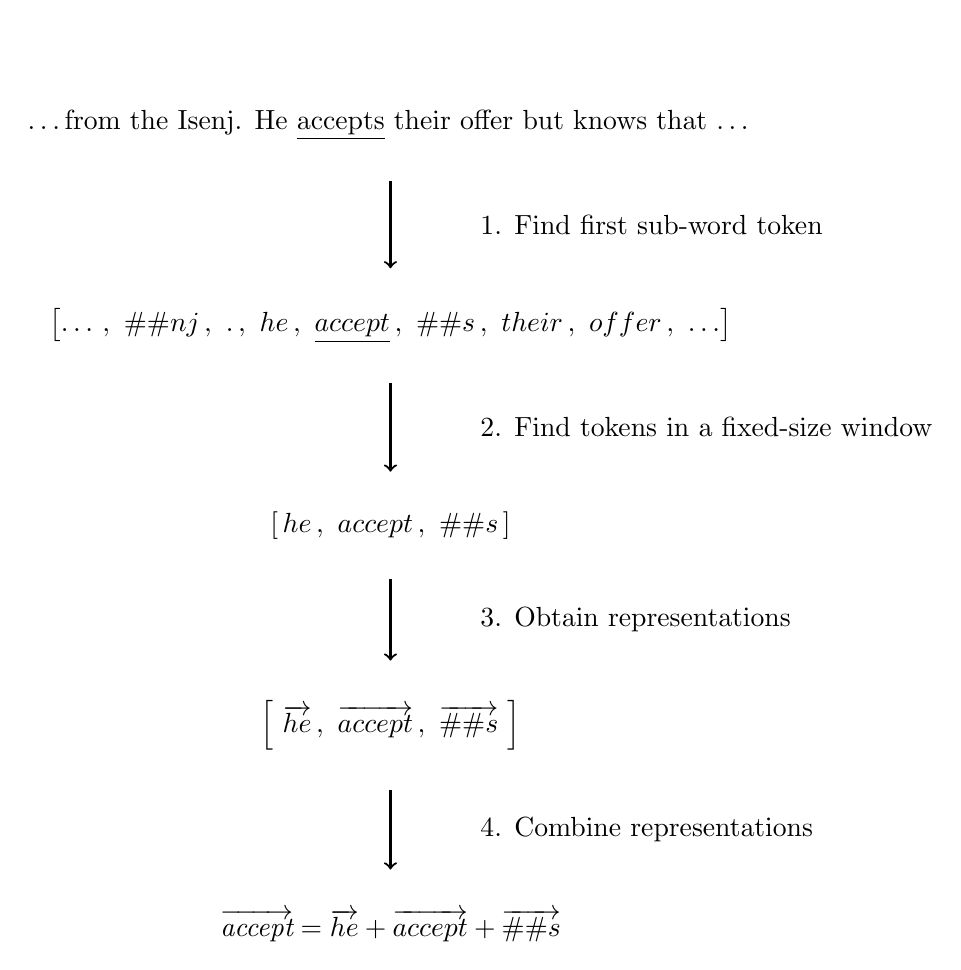
\begin{tikzpicture}[
      node distance = 1in,
      every node/.style = {
          inner sep = 0,
          outer sep = 0.2in
        }
    ]
    \node [label] (a) {
      \dots from the Isenj\period{} He \underline{accepts} their offer but knows that \dots
    };
    \node [label, below of=a] (b) {$\left[
          \dots\,,\
          \text{\#\#nj}\,,\
          \period{}\,,\
          \text{he}\,,\
          \text{\underline{accept}}\,,\
          \text{\#\#s}\,,\
          \text{their}\,,\
          \text{offer}\,,\
          \dots
          \right]$};
    \node [label, below of=b] (c) {$\left[
          \,
          \text{he}\,,\
          \text{accept}\,,\
          \text{\#\#s}
          \,
          \right]$};
    \node [label, below of=c] (d) {$\left[
          \
          \ora{\text{he}}\,,\
          \ora{\text{accept}}\,,\
          \ora{\text{\#\#s}}
          \
          \right]$};
    \node [label, below of=d] (e) {$
        \ora{\textit{accept}} =
        \ora{\text{he}} +
        \ora{\text{accept}} +
        \ora{\text{\#\#s}}
      $};
    \draw [thick, ->] (a) -- (b) node[midway, right=0.25in] {1. Find first sub-word token};
    \draw [thick, ->] (b) -- (c) node[midway, right=0.25in] {2. Find tokens in a fixed-size window};
    \draw [thick, ->] (c) -- (d) node[midway, right=0.25in] {3. Obtain representations};
    \draw [thick, ->] (d) -- (e) node[midway, right=0.25in] {4. Combine representations};
  \end{tikzpicture}
  \caption{A schematic of the procedure used to obtain a contextualised representation
    of a target word from pre-trained static or contextual embeddings. In this example,
    the target word is ``accept'', the window size is one (either side of the target
    word), and the composition operation is addition.}
\end{figure}

\begin{figure}
  \label{fig:language-models}
  \centering
  \begin{tabular}{lcccc}
    Model name & English    & Finnish    & Croatian   & Slovene
    \\
    \hline
    \texttt{EMBEDDIA/crosloengual-bert}\textsuperscript{1}
               & \checkmark & \checkmark & \checkmark & \checkmark
    \\
    \texttt{TurkuNLP/bert-base-finnish-cased-v1}\textsuperscript{2}
               &            & \checkmark &            &
    \\
    \texttt{TurkuNLP/bert-base-finnish-uncased-v1}\textsuperscript{2}
               &            & \checkmark &            &
    \\
    \texttt{TurkuNLP/bert-large-finnish-cased-v1}\textsuperscript{2}
               &            & \checkmark &            &
    \\
    \texttt{bert-base-cased}
               & \checkmark &            &            &
    \\
    \texttt{bert-base-multilingual-cased}
               & \checkmark & \checkmark & \checkmark & \checkmark
    \\
    \texttt{bert-base-multilingual-uncased}
               & \checkmark & \checkmark & \checkmark & \checkmark
    \\
    \texttt{bert-base-uncased}
               & \checkmark &            &            &
    \\
    \texttt{bert-large-cased}
               & \checkmark &            &            &
    \\
    \texttt{bert-large-cased-whole-word-masking}
               & \checkmark &            &            &
    \\
    \texttt{bert-large-uncased}
               & \checkmark &            &            &
    \\
    \texttt{bert-large-uncased-whole-word-masking}
               & \checkmark &            &            &
    \\
    \texttt{classla-bcms-bertic}\textsuperscript{3}
               &            &            & \checkmark &
  \end{tabular}
  \caption{The pre-trained models available via the HuggingFace \emph{Transformers}
    library \parencite{Wolf2020} that I chose to evaluate for each language. The
    corresponding references are
    \textsuperscript{1}\textcite{Ulcar2020},
    \textsuperscript{2}\textcite{Virtanen2019},
    \textsuperscript{3}\textcite{Ljubesic2021}, and
    \textcite{Devlin2019} otherwise.}
\end{figure}

Originally, it would not have been possible to optimise a parameterised model for the
task except by reference to a separate dataset; therefore, I chose to focus on the
application of pre-trained static and contextual embeddings.
The basic procedure of the methods that I evaluated is as follows.
For each pair of target words and each of the two contexts in which they appear, I
obtained a contextualised representation of a target word by:
finding the index of the target word's first sub-word token within the tokens of the target word's context;
finding the tokens within a fixed-size window around the target word's first token;
obtaining the embeddings of the tokens in the window; and
combining the the embeddings to produce a single representation of the target word.

In all cases, the tokenization was performed by and the embeddings were obtained from
pre-trained models available via the HuggingFace \emph{Transformers} library
\parencite{Wolf2020}.
The models that I evaluated for each language are given in Table~\ref{fig:language-models}.
For the static-embedding variants of the procedure, I used the models' input embeddings;
for the contextual-embedding variants, I used the models' outputs.
Several of the submissions to SemEval-2020 Task 3 used a combination of the weights of a
Transformer model's hidden states \parencites[e.g.,][276]{Gamallo2020}[3]{Pessutto2020}[4]{Hettiarachchi2021}; a thorough comparison of the performance of variants
of this approach is beyond the scope of this paper.

Notably, the use of a sub-word vocabulary by these models
\parencite[e.g.,][4174]{Devlin2019} dictates that a target word may be represented by a
different number of tokens in each context.
As a result, the representations of a pair of target words may be different in each
context, even if they are static and the window size is zero.
This is the cause of the non-zero scores obtained by models of this kind
(Section~\ref{appendix:window-size}), particularly for the Finnish language.

Inspired by \textcite{Landauer1997}, \textcite{Kintsch2001}, and
\textcite{Mitchell2008}, I predominantly investigated the application of element-wise
addition and multiplication as composition operations.
However, preliminary experiments indicated that multiplication performed poorly across
all languages, models, and window sizes; hence, it was discarded before the final
analysis.
Additionally, I chose to evaluate the concatenation (`stacking') of embeddings.
In the case that the number of embeddings was fewer than the context-window size, i.e.,
the target word was close to the beginning or the end of its context, I right-padded the
concatenated embedding with zeros to obtain contextual embeddings of equal length.
